%This is a experiment example of ZhengXiaoyang's experiment report template

\documentclass[UTF8]{ctexart}
 
\usepackage{amsmath}
\usepackage{cases}
\usepackage{cite}
\usepackage{xeCJK}
\usepackage{graphicx}
\usepackage{siunitx}
\usepackage[margin=1in]{geometry}
\geometry{a4paper}
\usepackage{fancyhdr}
\pagestyle{fancy}
\fancyhf{}

\graphicspath{{picture/}}





\title{观察一维驻波实验预习报告}
\author{郑晓旸}
\date{\today}
\pagenumbering{arabic}

\begin{document}
%这里是文件的开头
\fancyhead[L]{郑晓旸}
\fancyhead[C]{一维驻波}
\fancyfoot[C]{\thepage}

\maketitle
\tableofcontents
\newpage

\section{实验目的}
    \begin{enumerate}
        \item 加深对驻波、本征频率和本征模式概念的理解。
        \item 掌握测量弦上驻波的产生和测量方法。
        \item 观察弹簧上的纵波并测量其波速。
    \end{enumerate}

\section{实验仪器}
\begin{enumerate}
    \item 细绳
    \item 弹簧 
    \item 数字拉力计 
    \item 米尺 
    \item 机械波驱动器 
    \item 压电传感器 
    \item 正弦信号发生器 
    \item 示波器
\end{enumerate}

\section{实验原理}

\subsection{一维波动方程}

\subsubsection{弦上横波的波动方程}

如图\ref{fig:string_wave}所示,考虑一根两端受恒定张力$T$拉紧的轻质弦,设其线密度为$\rho$。取弦的平衡位置为$x$轴,令$u(x,t)$表示弦上质点在$t$时刻相对平衡位置的横向位移。
\\
\begin{figure}[htbp]
\centering
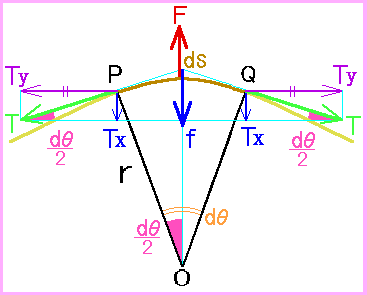
\includegraphics[width=0.4\textwidth]{string_wave.png}
\caption{弦上横波示意图}
\label{fig:string_wave}
\end{figure}
\\
考虑弦上$[x, x+\Delta x]$一小段,它受到两个相反方向的张力$\vec{T}$作用,合力在$y$方向的分量为
\begin{equation}
F_y = T\sin\theta(x+\Delta x) - T\sin\theta(x) \approx T\left(\frac{\partial u}{\partial x}\bigg|_{x+\Delta x} - \frac{\partial u}{\partial x}\bigg|_x\right) = T\frac{\partial^2u}{\partial x^2}\Delta x
\end{equation}

这一小段弦的质量为$\rho\Delta x$,根据牛顿第二定律$F_y = \rho\Delta x \frac{\partial^2u}{\partial t^2}$,整理得
\begin{equation}
\frac{\partial^2u}{\partial t^2} = \frac{T}{\rho}\frac{\partial^2u}{\partial x^2}
\end{equation}

令$v^2 = T/\rho$,这就是弦上横波满足的波动方程
\begin{equation}
\frac{\partial^2u}{\partial t^2} = v^2\frac{\partial^2u}{\partial x^2}
\label{eq:wave_eq_string}
\end{equation}

\subsubsection{弹簧上纵波的波动方程}

如图\ref{fig:spring_wave}所示,考虑一根劲度系数为$k$、未拉伸长度为$L$的轻质弹簧,在两端施加恒定拉力使其伸长到$L'$。取弹簧的平衡位置为$x$轴,令$u(x,t)$表示弹簧上质点在$t$时刻相对平衡位置的纵向位移。
\\
\begin{figure}[htbp]
\centering
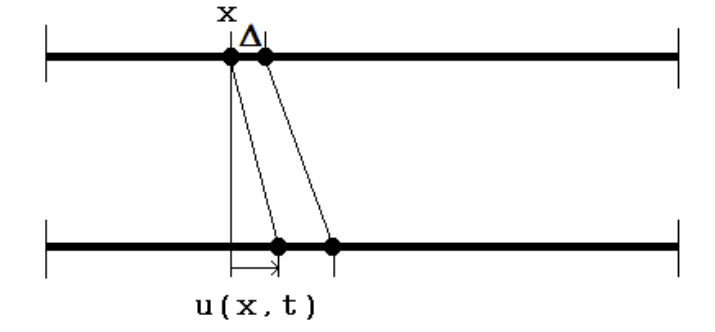
\includegraphics[width=0.5\textwidth]{spring_wave.png}
\caption{弹簧上纵波示意图}
\label{fig:spring_wave}
\end{figure}

考虑弹簧上$[x, x+\Delta x]$一小段,它两端的伸长量分别为$u(x+\Delta x, t)-u(x,t)$和$u(x,t)-u(x-\Delta x,t)$,根据胡克定律,两端的弹力大小分别为$k\frac{L}{L'}[u(x+\Delta x, t)-u(x,t)]$和$k\frac{L}{L'}[u(x,t)-u(x-\Delta x,t)]$。这一小段弹簧质量为$\rho\Delta x$,根据牛顿第二定律
\begin{equation}
\rho\Delta x\frac{\partial^2u}{\partial t^2} = k\frac{L}{L'}\left[u(x+\Delta x, t) - 2u(x,t) + u(x-\Delta x,t)\right]
\end{equation}

当$\Delta x \to 0$时,上式化为
\begin{equation}
\frac{\partial^2u}{\partial t^2} = \frac{kL}{\rho L'}\frac{\partial^2u}{\partial x^2}
\end{equation}

令$v^2 = \frac{kL}{\rho L'}$,得到弹簧上纵波的波动方程
\begin{equation}
\frac{\partial^2u}{\partial t^2} = v^2\frac{\partial^2u}{\partial x^2}
\label{eq:wave_eq_spring}
\end{equation}

\subsection{驻波和本征模式}

对于两端固定的有限弦或弹簧,设其长度为$L$,边界条件为$u(0,t)=u(L,t)=0$。此时波动方程(\ref{eq:wave_eq_string})和(\ref{eq:wave_eq_spring})的解为驻波
\begin{equation}
u(x,t) = A_n \sin(\frac{n\pi}{L}x)\cos(\omega_nt+\phi_n), \quad n=1,2,3,\cdots
\label{eq:standing_wave}
\end{equation}
其中$A_n$为第$n$阶驻波的振幅,$\phi_n$为初相位,本征角频率$\omega_n$满足
\begin{equation}
\omega_n = \frac{n\pi v}{L} = n\omega_1, \quad n=1,2,3,\cdots
\label{eq:eigen_freq}
\end{equation}

对应的本征函数$\sin\left(\frac{n\pi}{L}x\right)$称为第$n$阶本征模式,它在弦或弹簧上形成$n$个驻波波腹。相邻两个波腹之间的点称为波节点,其位移恒为零。

\subsection{共振与色散关系}

在实验中,我们通过在一端施加正弦驱动$u(0,t)=A\cos\omega t$激发弦或弹簧的振动。当驱动频率$\omega$接近某一阶本征频率$\omega_n$时,会发生共振,此时对应的本征模式振幅最大,远大于其他模式。因此通过扫描驱动频率,观察共振现象,就可以测量系统的本征频率。

另一方面,由(\ref{eq:eigen_freq})式可知,本征频率$\omega_n$与对应的波数$k_n=\frac{n\pi}{L}$满足线性关系
\begin{equation}
\omega_n = vk_n
\label{eq:dispersion}
\end{equation}

这表明弦上的横波和弹簧上的纵波都是无色散的,相速度等于群速度,等于波速$v$。通过测量一系列本征频率$\omega_n$和波数$k_n$,就可以验证色散关系(\ref{eq:dispersion}),并求出波速$v$。

\subsection{实验目的}

基于以上原理,本实验的目的可以归纳为:
\begin{enumerate}
\item 观察和测量弦上横波及弹簧上纵波的驻波模式,理解本征模式和本征频率的概念;
\item 通过共振法测量弦和弹簧的一系列本征频率,验证色散关系,求出波速;
\item 研究弦上横波的波速与张力、线密度的关系,验证波速公式$v=\sqrt{T/\rho}$;
\item 研究弹簧上纵波的波速与弹簧劲度系数、质量等参量的关系,验证波速公式$v=L\sqrt{k/m}$。
\end{enumerate}

\section{实验过程与实验数据}
\subsection{弦上驻波实验}
\begin{enumerate}
\item 搭建实验装置,调节支架位置,使弦保持水平,并用拉力计控制其张力。
\item 调节信号发生器输出频率,观察弦的振动情况。当出现清晰的驻波时,记录此时的频率,即某一阶本征频率$f_n$。
 记录得到长度为$L=\SI{700}{\milli \meter}$,拉力为$F = \SI{0.529}{\newton}$的弦上驻波的本征频率与阶数的关系为:
 \begin{table}[htbp]
    \centering
\begin{tabular}{|l|l|}
   
f(\SI{}{\hertz}) &n\\
\hline 
47.5&1\\
95.7&2\\
146.7&3\\
195.2&4\\
244.3&5\\
\end{tabular}
\end{table}
\\
基本符合基频与倍频之间的倍数关系。
\item 固定弦的张力,调节激励频率,得到各个本征频率的波长$\lambda_n$和波数$k_n$。并计算对应的$k_n$,最后作色散关系曲线$\omega \sim k$。
\\
\begin{figure}[htbp]
    \centering
    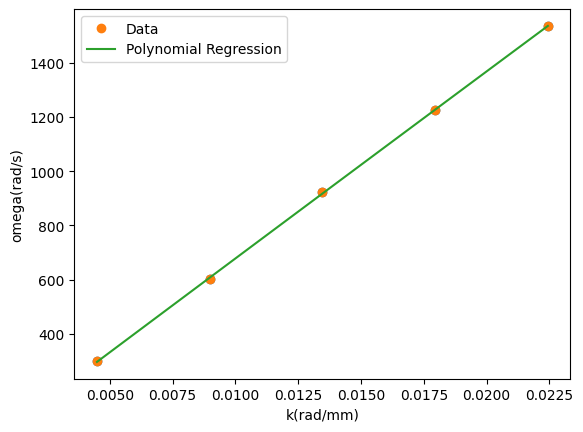
\includegraphics[width=0.6\textwidth]{dispersion_curve.png}
    \caption{色散关系曲线}
    \label{fig:dispersion_curve}
\end{figure}
\\
在这里我们使用二次多项式进行回归,得到回归系数:$ C_1 = 69454.0;C_2 = -15.1; r^2 = 0.99994$可见,色散关系高度线性,高阶量极小,且相关性极高。
\item 改变弦的张力,重复上述测量,研究波速$v$与张力$T$的关系。使用方程$v = a + \sqrt{b * T}$进行回归,得到。
\begin{figure}[htbp]
    \centering
    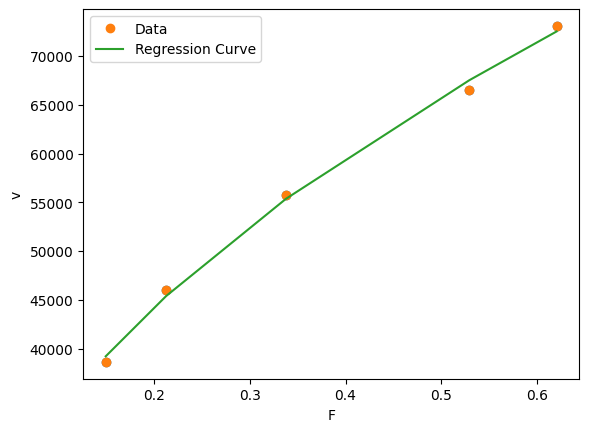
\includegraphics[width=0.6\textwidth]{tension_vs_velocity.png}
    \caption{拉力与波速关系图}
    \label{fig:tension_vs_velocity}
\end{figure}
\\回归结果为:$a = 6.98e3; b =  6.93e9 ; r^2 =0.99 $可明显观察到波速与张力的平方根成线性关系。

\end{enumerate}
\subsection{弹簧上驻波实验}
\begin{enumerate}
\item 将弹簧的一端固定,另一端连接机械波驱动器。调节弹簧的拉伸长度。
\item 从低频开始扫描驱动频率,观察弹簧的振动情况。当出现波节点清晰可见、其它部位运动模糊的现象时,即为共振。记录此时的频率$f_n$。
\item 记录得到本征频率为如下表格所示:
\\
\begin{table}[htbp]
    \centering
\begin{tabular}{l|l|l}
L&n&f\\
\hline
700&3&24.1\\
700&4&35.53\\
700&5&39.36\\
700&6&47.3\\
700&7&55.24\\
700&8&63.5\\
\end{tabular}
\end{table}
\\
\\可以发现,本征频率与阶数之间关系近似为线性关系。
\begin{figure}[htbp]
    \centering
    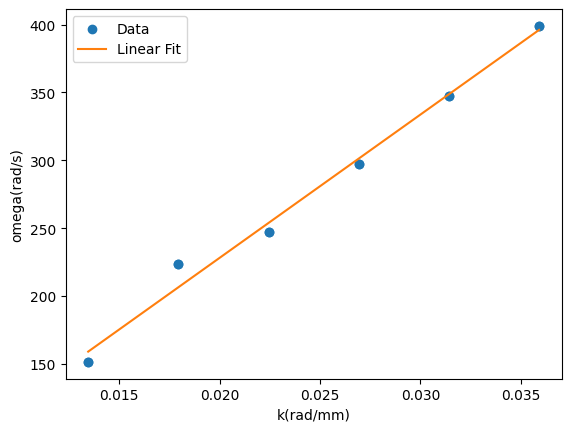
\includegraphics[width=0.6\textwidth]{output.png}
    \caption{弹簧纵波的色散关系}
    \label{fig:disp}
\end{figure}
其中$r^2 = 0.98$,拟合效果较差,这有可能是由于弹簧在振动时与固定部分之外的元件产生共振导致本征频率发生了偏移。
\end{enumerate}
\end{document}
